\documentclass[12pt]{article}
\usepackage[utf8]{inputenc}
\usepackage{amsmath}
\usepackage{mathrsfs}
\usepackage{amssymb}
\usepackage{amsfonts}

\DeclareMathOperator{\logit}{logit}
\DeclareMathOperator*{\argmax}{arg\,max}
\DeclareMathOperator*{\argmin}{arg\,min}

\usepackage[
    a4paper,
    left = 2.5cm,
    right = 2.5cm,
    top = 2.5cm,
    bottom = 2.5cm
]{geometry}

\usepackage{graphicx}
\usepackage[headings]{fullpage}
\usepackage{hyperref}
\usepackage{fancyhdr}
 %For aligned formulas
 \usepackage{IEEEtrantools}
\usepackage{listings} %Source code listings https://en.wikibooks.org/wiki/LaTeX/Source_Code_Listings

\lstset{
    language=R, %You can always set to another language
    breaklines,
    deletekeywords={category},
    basicstyle=\ttfamily\footnotesize,
    otherkeywords={!,!=,~,\$,*,\&,\%/\%,\%*\%,\%\%,<-,<<-},
    literate={~}{$\sim$}1 {<-}{{$\gets$}}1
}

\usepackage[
    backend=biber,
    style=apa,
    maxcitenames=2,
    mincitenames=1,
    sorting=ynt
    ]{biblatex}
\addbibresource{bibfile.bib}

\setlength{\headheight}{15pt}
\pagestyle{fancy}
\fancyhf{}
\rhead{YOUR NAMES} % Fill in your name
%\lhead{Bayesian Statistics \& Probabilistic Machine Learning---Project Report}
\rfoot{Page \thepage}


\begin{document}

\begin{titlepage}
        \centering % Center all text
        \vspace*{\baselineskip} % White space at the top of the page
        
        {\huge YOUR TITLE}\\[0.2\baselineskip] % Title
        
        
        \vspace*{\baselineskip}
        
        {\Large --- Project Report ---\\
          Advanced Bayesian Data Analysis\\[\baselineskip]} % Tagline(s) or further description
        \vspace*{\baselineskip}
        
        {\LARGE YOUR NAMES\\[\baselineskip]} % Editor list  
        
        \vspace*{\baselineskip}

        \vfill
        
        \today \par % Location and year
        
        \vspace*{\baselineskip}

        {\itshape TU Dortmund University\par} % Editor affiliation
    \end{titlepage}

\clearpage

\section{Introduction}
This is a template for the project report in the course Advanced Bayesian Data Analysis.
Fill in your title and names for the title page and header and follow the general structure. You don't have to use multiple chapters or sections at all for this short report, but if you do, don't go further than subsections--- \textcite{feynman1963lnphysics} didn't need to\ldots

Some examples on how to use \LaTeX{} are shown below. If you want to reference something, you can do it as so:
\textcite{mcelreath2016statistical}.

\subsection{Images}
\begin{figure}
    \begin{center}
    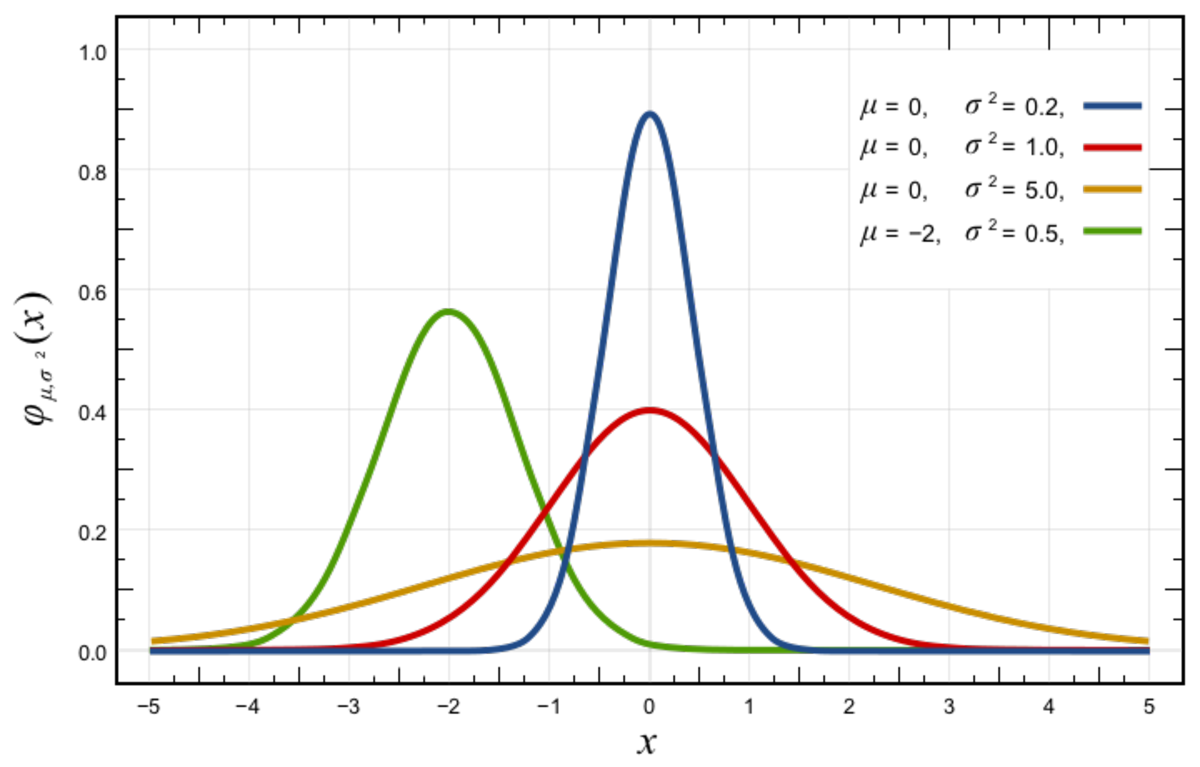
\includegraphics[width=0.5\textwidth]{figures/Normal_Distribution_PDF.pdf} %try to never force a figure placement
    \caption{Probability density function for the Normal distribution. The red curve is the standard normal distribution. [By Inductiveload - self-made, Mathematica, Inkscape, Public Domain, \url{https://commons.wikimedia.org/w/index.php?curid=3817954}]}
    \label{fig:normal_sample}
    \end{center}
\end{figure}

This is an example for how to insert images into your document. When talking about a figure, you should always point out which one you mean, i.e., ``As you can see in Figure~\ref{fig:normal_sample}.''

\subsection{Tables}
A table has a caption \textit{above} the table as in Table~\ref{tab:my_label}.

\begin{table} %You can place [h] immediately after \begin{table} to force the placement of the table. Generally speaking never do that---LaTeX usually places them in a sane way!
    \centering
    \caption{My caption.}
    \label{tab:my_label}
    \begin{tabular}{c|l} % l, r, and c justified inside cells.
        \hline
         Poisson & $\lambda$ \\ % Always end a line with \\
         Normal &  $\mu$ and $\sigma$\\ 
        \hline
    \end{tabular}
\end{table}

\subsection{Formulas}
This is a small example for how to include formulas into your document. $a^2 + b^2 = c^2$ will inline a formula, while
$$c \leq a + b$$
will give the formula its own line.

\subsection{Formulas}
You also might want to write out models:

{\footnotesize % you align formulas using & 
\begin{IEEEeqnarray*}{rCl}
\mathrm{L}_i & \sim & \mathrm{Binomial}(n_i,p_i)\\
\mathrm{logit}(p_i) & = & \alpha_{\mathrm{SUBJECT}[i]} + (\beta_P + \beta_{PC}C_i)P_i\\
\alpha_{\mathrm{SUBJECT}} & \sim & \mathrm{Normal}(0,10) \\
\beta_P & \sim & \mathrm{Normal}(0,10)\\
\beta_{PC} & \sim & \mathrm{Normal}(0,10)
\end{IEEEeqnarray*}
}


\subsection{Source code}
Of course, formatting source code is always nice.
\begin{lstlisting}
m <- map(
    alist(
        height ~ dnorm(mu, sigma),
        mu <- a + b*weight,
        a ~ dnorm(0, 100),
        b ~ dnorm(0, 10),
        sigma ~ dunif(0, 50) 
    ), 
    data=d2)
\end{lstlisting}

\subsection{Math fonts}
Different math fonts are also available to you:

$\mathrm{ABCDE abcde 1234}$

$\mathit{ABCDE abcde 1234}$

$\mathnormal{ABCDEabcde1234}$

$\mathcal{ABCDE abcde 1234}$

$\mathscr{ABCDE abcde 1234}$

$\mathfrak{ABCDE abcde 1234}$

$\mathbb{ABCDE abcde 1234}$

\printbibliography

\end{document}
